%%%%%%%%%%%%%%%%%%%%%%%%%%%%%%%%%%%%%%%%%%%%%%%%%%%%%%%%%%%%%%%%%%%%%%%%%%%%%%%%%%%%%
%%%%%%%%%%%%%%%%%%%%%%%%%%%%%%%%%%%%%%%%%%%%%%%%%%%%%%%%%%%%%%%%%%%%%%%%%%%%%%%%%%%%%

\setbeamercolor{block title}{bg=white, fg=black}
\setbeamercolor{body}{bg=blue!20}

\begin{frame}
	\frametitle{Static analysis}

	\begin{block}{}
	\centering
	Static program analysis is the analysis of computer software which is performed without actually executing programs
	\end{block}
		
	\begin{figure}
	
\includegraphics[width=70mm]{image/staticAnalysis}
	\end{figure}	
	
\end{frame}

%%%%%%%%%%%%%%%%%%%%%%%%%%%%%%%%%%%%%%%%%%%%%%%%%%%%%%%%%%%%%%%%%%%%%%%%%%%%%%%%%%%%%
%%%%%%%%%%%%%%%%%%%%%%%%%%%%%%%%%%%%%%%%%%%%%%%%%%%%%%%%%%%%%%%%%%%%%%%%%%%%%%%%%%%%%


\begin{frame}
	\frametitle{Performance problem}
	\begin{itemize}
		\item Most static analyses have big problems with performance
		\item Our bounded model checking tool Borealis is not an exception
		\item We decided to try \textit{scaling} Borealis to multiple cores
	\end{itemize}
\end{frame}


%%%%%%%%%%%%%%%%%%%%%%%%%%%%%%%%%%%%%%%%%%%%%%%%%%%%%%%%%%%%%%%%%%%%%%%%%%%%%%%%%%%%%
%%%%%%%%%%%%%%%%%%%%%%%%%%%%%%%%%%%%%%%%%%%%%%%%%%%%%%%%%%%%%%%%%%%%%%%%%%%%%%%%%%%%%

\begin{frame}
\frametitle{Bounded model checking algorithm}
	\begin{figure}
	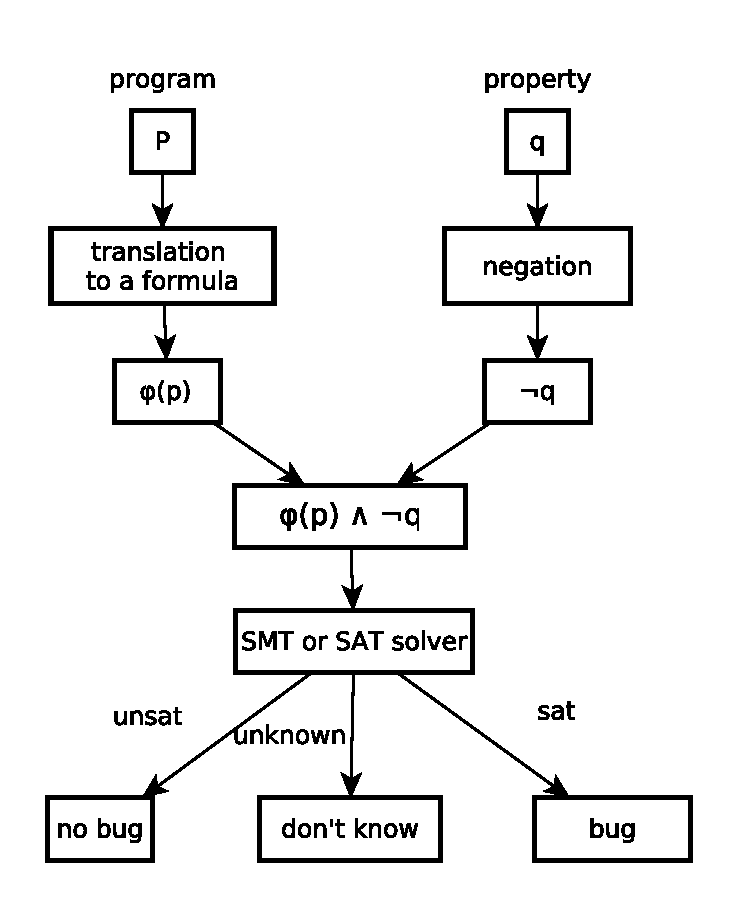
\includegraphics[width=65mm]{image/BMC}
	\end{figure}	
\end{frame}


\begin{frame}[fragile]\frametitle{Verification example} 
\center 
\begin{columns} 
\column{0.5\textwidth} 
\center{Program:} 
\begin{lstlisting}[style=crs_cpp] 
int x; 
int y=8,z=0,w=0; 
if (x) 
	z = y - 1; 
else 
	w = y + 1; 
assert (z == 7 || w == 9) 
\end{lstlisting} 
\column{0.5\textwidth} 
\center{Constraints:} 
\begin{lstlisting}[style = crs_llvm] 
y = 8, 
z = x ? y -1 : 0, 
w = x ? 0 : y + 1, 
z != 7, 
w != 9 
\end{lstlisting} 
\end{columns} 
	\begin{block}{}
	\centering
UNSAT. Assert always true
	\end{block}
\end{frame} 


%%%%%%%%%%%%%%%%%%%%%%%%%%%%%%%%%%%%%%%%%%%%%%%%%%%%%%%%%%%%%%%%%%%%%%%%%%%%%%%%%%%%%
%%%%%%%%%%%%%%%%%%%%%%%%%%%%%%%%%%%%%%%%%%%%%%%%%%%%%%%%%%%%%%%%%%%%%%%%%%%%%%%%%%%%%


\begin{frame}[fragile]\frametitle{Verification example} 
\center 
\begin{columns} 
\column{0.5\textwidth} 
\center{Program:} 
\begin{lstlisting}[style=crs_cpp] 
int x; 
int y=8,z=0,w=0; 
if (x) 
	z = y - 1; 
else 
	w = y + 1; 
assert (z == 5 || w == 9) 
\end{lstlisting} 
\column{0.5\textwidth} 
\center{Constraints:} 
\begin{lstlisting}[style = crs_llvm] 
y = 8, 
z = x ? y -1 : 0, 
w = x ? 0 : y + 1, 
z != 5, 
w != 9 
\end{lstlisting} 
\end{columns} 
	\begin{block}{}
	\centering
SAT. Program contains a bug \\
Counterexample: y = 8, x = 1, w = 0, z = 7
	\end{block}
\end{frame}


%%%%%%%%%%%%%%%%%%%%%%%%%%%%%%%%%%%%%%%%%%%%%%%%%%%%%%%%%%%%%%%%%%%%%%%%%%%%%%%%%%%%%
%%%%%%%%%%%%%%%%%%%%%%%%%%%%%%%%%%%%%%%%%%%%%%%%%%%%%%%%%%%%%%%%%%%%%%%%%%%%%%%%%%%%%

\begin{frame}
	\frametitle{Borealis}
	
	\begin{figure}
	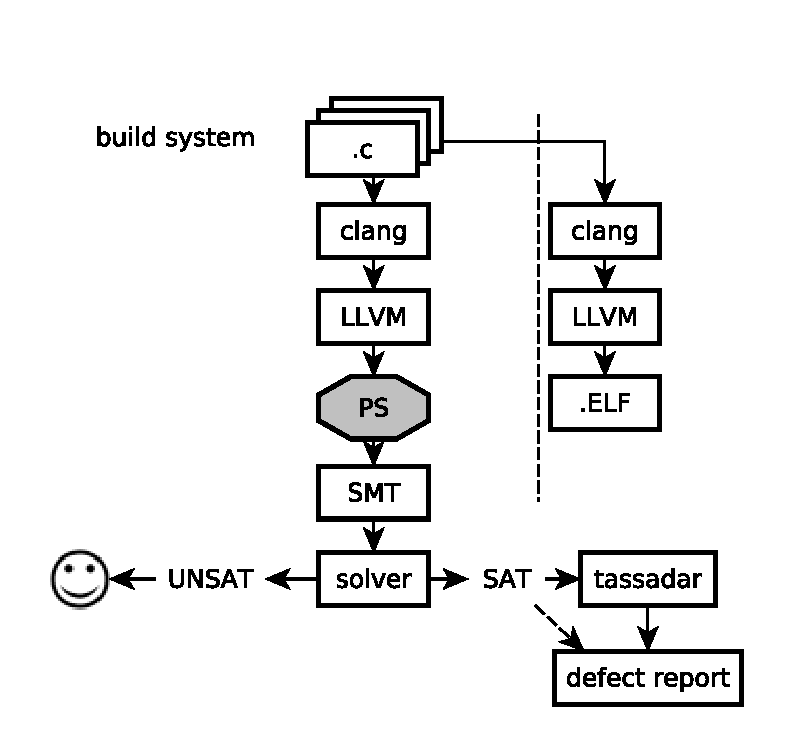
\includegraphics[width=80mm]{image/BorealisOverview}
	\end{figure}	
	
\end{frame}

%%%%%%%%%%%%%%%%%%%%%%%%%%%%%%%%%%%%%%%%%%%%%%%%%%%%%%%%%%%%%%%%%%%%%%%%%%%%%%%%%%%%%
%%%%%%%%%%%%%%%%%%%%%%%%%%%%%%%%%%%%%%%%%%%%%%%%%%%%%%%%%%%%%%%%%%%%%%%%%%%%%%%%%%%%%

\begin{frame}
	\frametitle{Program representation}
	\begin{figure}
	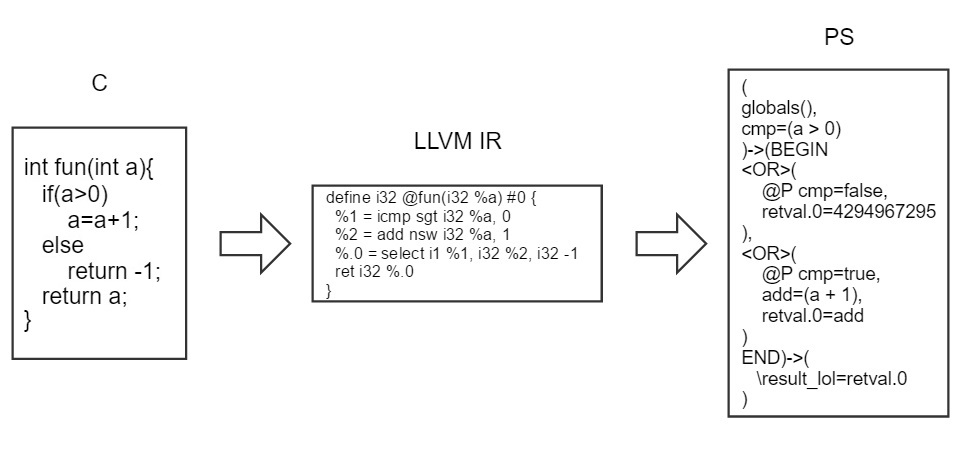
\includegraphics[width=110mm, keepaspectratio]{image/PSdef}
	\end{figure}
\end{frame}


%%%%%%%%%%%%%%%%%%%%%%%%%%%%%%%%%%%%%%%%%%%%%%%%%%%%%%%%%%%%%%%%%%%%%%%%%%%%%%%%%%%%%
%%%%%%%%%%%%%%%%%%%%%%%%%%%%%%%%%%%%%%%%%%%%%%%%%%%%%%%%%%%%%%%%%%%%%%%%%%%%%%%%%%%%%

\setbeamercolor{block title}{bg=white, fg=black}
\setbeamercolor{block body}{bg=blue!20}
\begin{frame}
\frametitle{Problem}
	\begin{block}{}
		\centering
		The huge number of SMT queries involved in checking process
	\end{block}
\setbeamercolor{block body}{bg=red!20}
	\begin{block}{}
		\centering
		We try to scale Borealis to multiple cores on our RSC Tornado
	\end{block}
\end{frame}

%%%%%%%%%%%%%%%%%%%%%%%%%%%%%%%%%%%%%%%%%%%%%%%%%%%%%%%%%%%%%%%%%%%%%%%%%%%%%%%%%%%%%
%%%%%%%%%%%%%%%%%%%%%%%%%%%%%%%%%%%%%%%%%%%%%%%%%%%%%%%%%%%%%%%%%%%%%%%%%%%%%%%%%%%%%

\begin{frame}
\frametitle{RSC Tornado supercomputer}
\begin{itemize}
\item 712 dual-processor nodes with 1424 Intel Xeon E5-2697
\item 64 GB of DDR4 RAM and local 120 GB SSD storage
\item 1 PB Lustre storage
\item InfiniBand FDR, 56 Gb/s
\end{itemize}
\end{frame}

%%%%%%%%%%%%%%%%%%%%%%%%%%%%%%%%%%%%%%%%%%%%%%%%%%%%%%%%%%%%%%%%%%%%%%%%%%%%%%%%%%%%%
%%%%%%%%%%%%%%%%%%%%%%%%%%%%%%%%%%%%%%%%%%%%%%%%%%%%%%%%%%%%%%%%%%%%%%%%%%%%%%%%%%%%%

\begin{frame}
\frametitle{Lustre storage}
\begin{itemize}
\item Parallel distributed file system
\item Highly scalable
\item Terabytes per second of I/O throughput
\item \textcolor{red}{Inefficient work with small files}
\end{itemize}
\end{frame}
